\documentclass{article}
\usepackage{tikz}
\usepackage{amsmath}
\usepackage{amssymb} 
\usepackage[a4paper]{geometry}
\usepackage{fancyhdr}
\pagestyle{fancy}
\lhead{Umkehrfunktionen}
\rhead{März 2025}
\begin{document}
\section{Umkehrfunktionen}
Die Funktion $f^{-1}(x)$ ist die Umkehrfunktion zu $f(x)$, wenn für alle Werte von $x \in \mathbb{R}$ die Gleichung $x = f^{-1}(f(x))$ gilt, heißt wenn die Berechnung von $f(x)$ Umgekehrt werden kann und mit einem gegebenen Ergebniss von $f(x)$ der dazugehörige Wert $x$ gefunden werden kann. \newline
Ist beispielsweise $f(1)=16 \implies f^{-1}(16)=1$. \newline
Eine Funktion $f$ kann nur eine Umkehrfunktion haben, wenn sie Eineindeutig ist, heißt es für jeden $y$ Wert nur genau einen $x$ gibt. Dies liegt vor, wenn die Funktion streng monoton Fallend oder Steigend ist. 
 
\subsection{Bestimmen}
Die Umkehrfunktion einer Funktion kann in wenigen Schritten einfach gefunden werden.
\begin{enumerate}
 \item Aufschreiben der gegebenen Funktion, wobei das $f(x)$ als Variable $y$ aufgeschrieben wird.
 \item Auflösen nach dem Eingangswert der gegebenen Funktion $x$ in abhängigkeit von $y$. 
 \item Das gefundene $x$ mit einem $f^{-1}$ ersetzen, das $y$ durch ein $x$ erstezen.
 \item \texttt{(optional)} Richtigkeit der gefundenen Umkehrfunktion mit Beispeilzahlen überprüfen. 
\end{enumerate}
 
\subsection{Umformungen}
Beim Auflösen nach dem $x$ können alle bereits bekannten algebraischen Umformungsregeln angewendet werden.
 
\begin{center}
\begin{tabular}{ |c|c| } 
\hline
 $y = x + r$ & $x = y - r$ \\
\hline
 $\rule{0pt}{4ex} \raisebox{1ex}{$y = x \cdot r$}$ & $\raisebox{1.1ex}{$x = \dfrac{y}{r}$}$ \\
\hline
 $\rule{0pt}{3ex} \raisebox{0.5ex}{$y = x^2$}$ & $\raisebox{0.5ex}{$x = \pm \sqrt[2]{y}$}$ \\
\hline
 $y = e^x$ & $x = \ln{y}$ \\
\hline
\end{tabular}
\end{center}  
Gibt es mehrere Lösungen bei der Umformung, gibt es auch mehrere Umkehrfunktionen, unterschieden mit einem Subskript. Ist beispielsweise $f(x)=x^2$, dann gibt es $f^{-1}_1=\sqrt{x}$ und $f^{-1}_2=-\sqrt{x}$.
 
\subsection{Zusammenhänge}
\begin{minipage}[t]{\dimexpr\textwidth-5cm}
 \vspace{0pt} 
 Die Umkehrfunktion verläuft genau so wie die gegebene Funktion, nur an der Achse $y=x$ gespiegelt. Zudem ist die Definitionsmenge einer Funktion die Wertemenge der zugehörigen Umkehrfunktion ist und umgekehrt. \newline
 Die Beispielfunktion ${f(x)=e^x}$ hat für ${\mathrm{D}=\{x \in \mathbb{R}\}}$ die ${\mathrm{W}=\{y \in \mathbb{R} \,\vert\, y> 0\}}$. Die dazugehörige Umkehrfunktion ${f^{-1}(x)=\ln{x}}$ hat dementsprechend für ${\mathrm{D}=\{x \in \mathbb{R} \,\vert\, x> 0\}}$ die ${\mathrm{W}=\{y \in \mathbb{R}\}}$.
\end{minipage}
\hfill
\begin{minipage}[t]{5cm}
  \centering
  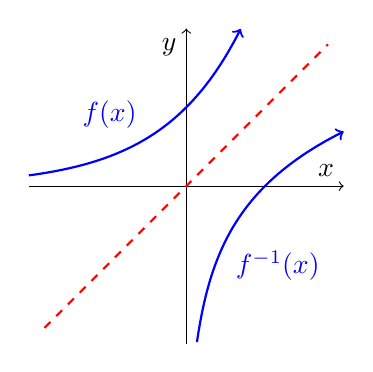
\begin{tikzpicture}[baseline=(current bounding box.north)]
  \draw[->] (-2,0) -- (2,0) node[above left] {$x$};
  \draw[->] (0,-2) -- (0,2) node[below left] {$y$};
  
  \draw[thick, dashed, red] (-1.8,-1.8) -- (1.8,1.8);
 
  \draw[->, blue, thick, domain=-2:ln(2), samples=100] 
            plot (\x, {e^(\x)}) node at (-0.5, {exp(-0.5)}) [above left] {$f(x)$};
  \draw[->, blue, thick, domain=e^-2:2, samples=100] 
            plot (\x, {ln{\x}}) node at (0.5, {ln(0.5)}) [below right] {$f^{-1}(x)$}; 
  \end{tikzpicture}
\end{minipage} 
 
\end{document}
 
 
 
 
